\documentclass[11pt]{article}
\usepackage{fullpage}
\usepackage{amsmath}
\usepackage{amssymb}
\usepackage{array}
\usepackage{graphicx}

\title{Econometric Homework 2}
\author{Tom Augspurger}
\begin{document}
\maketitle

\textbf{Problem 1:} Suppose $Y_{i}$ ~ i.i.d. $N(0, \sigma^{2}) i = 1, 2, \ldots, n$\\

\textbf{a.)}
\begin{align*}
    \sigma^{2} &= E[Y_{i}^{2}] - E^{2}[Y_{i}]\\
    &= E[Y_{i}^{2}]
\end{align*}

since $E[Y_{i}] = 0$, the square of the expectation is also zero.  So,

\begin{equation*}
    E\left[\frac{Y_{i}^{2}}{\sigma^{2}}\right] = E\left[\frac{\sigma^{2}}{\sigma^{2}}\right] = 1
\end{equation*}

\textbf{b.)} Let $W = (1/\sigma^{2})\sum_{i}^{n}Y_{i}^{2}$.  Show that $W$ is distributed according to $\chi_{n}^{2}$.

Let $X$ = $\frac{1}{\sigma^{2}} Y_{i}$.  We want to show that $X \thicksim N(0, 1)$.
First note that $X$ is a linear transformation of $Y$ with $a = 0$ and $b = \frac{1}{\sigma^{2}}$.  So $X \thicksim N(a + b\mu, b^{2}\sigma^{2})$. Simplifying $a + b\mu = 0 + \frac{1}{\sigma^{2}}0 = 0$, and $b^{2}\sigma^{2} = \frac{1}{\sigma^{4}}\sigma^{2} = \sigma^{2}$.  This gives us the desired result, $X \thicksim N(0, 1)$. Therefore, 
\[
    W = \sum_{i}^{n}X_{i}^{2} = (1/\sigma^{2})\sum_{i}^{n}Y_{i}^{2} \thicksim \chi^{2}(n)
\]\\

\textbf{c.)} Show that $E[W] = n$

$E[W] = E[(1/\sigma^{2}) \sum_{i}^{n}Y_{i}^{2}] = (1/\sigma^{2}) E[\sum_{i = 2}^{n}Y_{i}^{2}] = n\frac{\sigma^{2}}{\sigma^{2}} = n$\\


\textbf{d.)} We want to show that $V \equiv Y_{1} / \sqrt{\frac{\sum_{i}^{n}Y_{i}^{2}}{n - 1}}$\\

Let $W \equiv \frac{1}{\sigma^{2}}\sum_{i = 2}^{n}$.  Then $W \thicksim \chi^{2}(n - 1)$.

Let $Z \equiv (Y_{1} - \mu)/\sigma$.  Since $E(Y_{1}) = \mu$, $\mu = 0$, and $V(Y_{1}) = \sigma^{2}$, $Z \thicksim N(0, 1)$. So we have

\begin{align*}
    V &= Z/\sqrt{1 / \sigma^{2} \frac{W}{n - 1}}\\
    &= \frac{1}{\sigma}Y_{1} / (\frac{1}{\sigma}\frac{\sum_{i = 2}^{n} Y_{i}^{2}}{n - 1})\\
    &= Y_{1} / \sqrt{\frac{\sum_{i}^{n}Y_{i}^{2}}{n - 1}}
\end{align*}

so $V \thicksim$ $t_{n-1}$.\\


\textbf{Problem 2:} 

\textbf{a.)} Find $E[X], V[X], $and $Pr(A)$ where $A$ is the event $\{0.3 < X \leq 0.7\}$ for:
\begin{itemize}
    \item $X \thicksim$ Bernoulli(p):
    $E[x] = p = 0.5$
    $V(X) = p(1-p) = 0.25$
    $Pr(A) = 0$ since $ x \in \{0, 1\}$
    
    \item $X \thicksim N(0.5, 0.25)$
    $E[X] = \mu = 0.5$
    $V[X] = \sigma^{2} = 0.25$\\
    \begin{align*}
        Pr(A) &= Pr(\frac{0.3 - 0.5}{(1/16)} \leq Z \leq \frac{0.7 - 0.5}{(1/16)})\\
        &= 1 - 2 * Pr(Z \leq 3.2)\\
        &= 1 - 0.26 = 0.974
    \end{align*}
    
    \item $X \thicksim$ Exponential(2)
    $E[X] = \lambda^{-1} = \frac{1}{2}$
    $V(X) = \lambda^{-2} = \frac{1}{4}$
    \begin{align*}
        Pr(A) &= (1 - e^{-2(0.7)}) - (1 - e^{2(0.3)})\\
        &= 0.3221
    \end{align*}
\end{itemize}

\textbf{Problem 3:} $Y_{i} \thicksim i.i.d.\ N(10, 4)$.  Find $Pr(9.6 \leq \overline{Y} \leq 10.4)$.
Note that $\overline{Y} \thicksim N(\mu, \sigma^{2}/n)$.
\begin{itemize}
    \item n = 20.
    $|Z_{9.6}| = Z_{10.4} = \sqrt{20}\frac{9.6 - 10}{(2)} = .894427$
    so $Pr(9.6 \leq \overline{Y} \leq 10.4)) \approx 1 - 2(.1867) = .6266$
    
    \item n = 100
    $Z_{9.6} \approx -2.00$ so $Pr(9.6 \leq \overline{Y} \leq 10.4) \approx 1 - 2(.0228) = .9544$
    
    \item n = 1000
    $Z_{9.6} \approx -6.325$ so $Pr(9.6 \leq \overline{Y} \leq 10.4) \approx 0$\\

\end{itemize}
    
\textbf{b.)} Let $c > 0$.  $E[\overline{Y_{n}}] = 10$ and $V(\overline{Y_{n}}) = \sigma^{2}/n$ so lim $E[\overline{Y_{n}}] = 10$ and lim $V(\overline{Y_{n}}) = 0$.  This is an application of the LLN.

\textbf{c.)} This means that $\overline{Y_{n}}$ converges in mean square to $10$.  That is lim $E(\overline{Y_{n}} - c^{2}) = 0$ so if $A_{n} = \{|\overline{Y_{n}} - c| \ge \epsilon \}$, $0 \leq Pr(A_{n}) \leq E(\overline{Y_{n}} - c)^{2}/\epsilon^{2}$.  In the limit we have $0 \leq$ lim $ Pr(\overline{Y_{n}}) \leq 0$.  That is $\overline{Y} \thicksim\!\!\!\!\!^{{}^{p}} \ 10$.\\

\textbf{Problem 4} Let $\overline{X} \thicksim$ exponential($\lambda$). Let $\theta = E[X] = 1/\lambda$.  Let $U = 1/\overline{X}$.

\textbf{a.)} We want to show that plim $U = \lambda$  Using S1,
plim $\overline{X} = (1/\lambda)$ and $E[\overline{X}] = \theta \ \forall \ n$ so plim $U = 1/\overline{X} = 1/\theta = \lambda$.

\textbf{b.)} Find the limiting distribution of $\sqrt{n}(U - \lambda)$.
Since $X_{n} \thicksim$ exponential($\lambda$), $\sqrt{n}(\overline{X} - \theta)$ converges in distribution to $N(0, \theta^{2})$.  And since $U = 1/\overline{X}$ is continuously differentiable at $\theta$,

$\sqrt{n}(U - \lambda) \thicksim\!\!\!\!\!\!\!^{{}^{\textrm{ D}}} N(0, [U'(\theta)]^{2}\theta^{2})$, or alternativly

\[
\overline{X} \thicksim\!\!\!\!\!\!\!^{{}^{\textrm{ A}}}\  N(\theta, \theta^{-2}/n) \equiv \overline{X} \thicksim\!\!\!\!\!\!\!^{{}^{\textrm{ A}}}\ N(1/\lambda, \lambda^{2}/n)
\] 

\textbf{c.)} Approximate $Pr(U \leq 5/2)$ for $n = 16, \lambda = 2$.

$Pr(U \leq 5/2)$ normalizes to the probability that Z is less than $c^{*} = \sqrt{n}(\frac{5/2 - \mu}{\sigma}) = 4(\frac{(5/2 - 2)}{(1/2)}) = 1$.  From a standard normal table (or integration) we find that this is 0.8413.

\textbf{d.)}  For the exact $Pr(U \leq 5/2)$ first note that if $X \thicksim exp(\lambda)$ then $W \thicksim \chi^{2}(2n)$ where $W = 2n\lambda \overline{X}$.  So here we have that $W \thicksim \chi^{2}(32)$ and $W = 64\overline{X}$ or $\overline{X} = (1/64)W$

We want $Pr(U \leq 5/2) = Pr(1/ \overline{X} \leq 5/2) = Pr(\overline{X} \geq 2/5).$  Now substituting in $W$: $Pr(\overline{X} \geq 2/5) = Pr(W \geq 25.6) = .7810$\\


\textbf{Problem 5:}  The following table contains the results from a Monte Carlo simulation.  $X$ is a sample of 100 draws from a uniform distribution over $[0, 10]$. $Y$ is draw from a conditional distribution given by $E[Y_{i}|x_{i}] = 10 - x_{i}$, with a conditional variance of 25 for every $x_{i}$ (homoskedasticity).  $\overline{X}$ is the sample mean for the independent variable, $\overline{Y}$ is the mean of the sample means for the dependent variable.  That is the mean of the unconditional expectation of $Y$ over the 1000 simulations.  $\beta_{0}$ is the coefficient on the intercept and $beta_{1}$ is the coefficient on $X$. Finally, we have $s^{2}$, the conditional variance.
{
\setlength{\extrarowheight}{3pt}
    \begin{center}
        \begin{tabular}{ | c | c | c | c | c | c |}
            \hline
            & $\overline{X}$ & $\overline{Y}$ & $\beta_{0}$ & $\beta_{1}$ & $s^{2}$\\
            \hline
            Expected & 5 & 5 & 10 & -1 & 25\\
            \hline
            Observed & 5.083 & 4.917 & 10.009 & -1.002 & 24.912\\
            \hline
        \end{tabular}
    \end{center}
}

So we can see that the Monte Carlo simulation approximates the population distribution well.

\begin{figure}[htb]
    \centering
    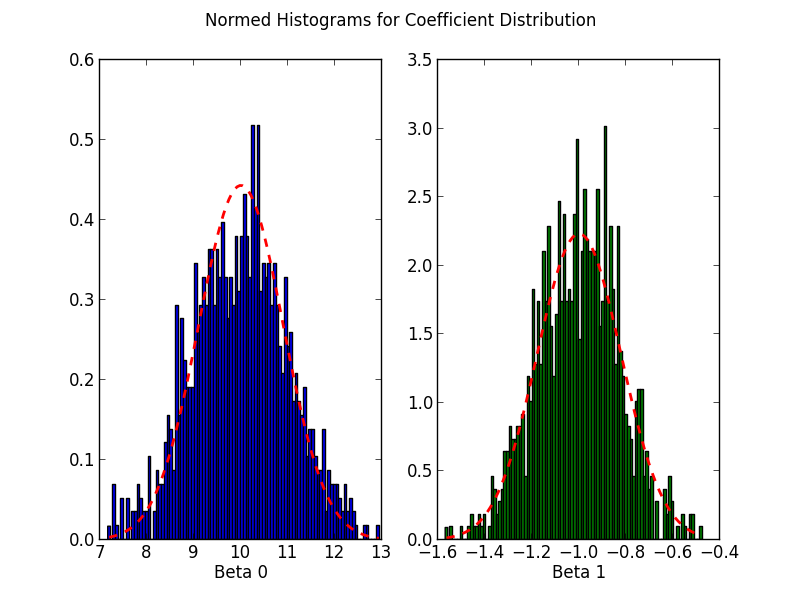
\includegraphics[scale = 0.5]{HW2Histograms}
\end{figure}













\end{document}